\documentclass[tikz,border=12pt]{standalone}
\usepackage[T1]{fontenc}
\usepackage{mathpazo}
\usepackage{amsmath,amssymb}
\usetikzlibrary{arrows.meta, positioning, calc, fit, decorations.pathreplacing}

\definecolor{stblue}{HTML}{7B97AD}
\definecolor{rwgold}{HTML}{B8995E}
\definecolor{sage}{HTML}{7A9A7E}
\definecolor{dkbrown}{HTML}{3D3530}
\definecolor{wmgray}{HTML}{7B7067}
\definecolor{cream}{HTML}{F9F6F0}
\definecolor{border}{HTML}{D4C9B8}
\definecolor{terracotta}{HTML}{C47A6A}
\definecolor{lavender}{HTML}{907EA0}

\begin{document}
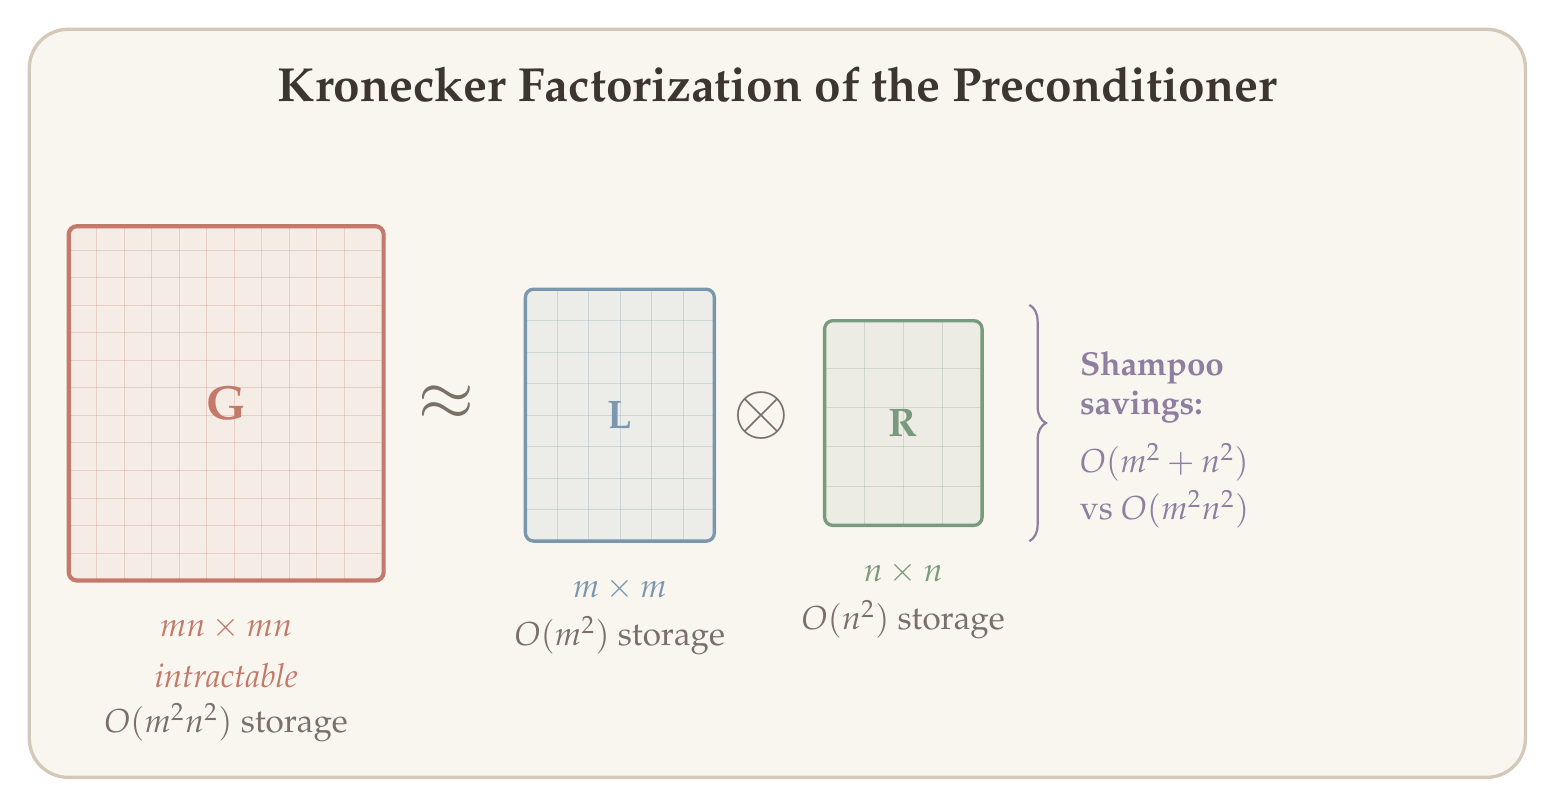
\begin{tikzpicture}[>={Stealth[length=4mm, width=3mm]}, line width=1.5pt]

% Background
\fill[cream, rounded corners=14pt] (-0.5,-2.0) rectangle (18.5,7.5);
\draw[border, line width=1.2pt, rounded corners=14pt] (-0.5,-2.0) rectangle (18.5,7.5);

% Title
\node[text=dkbrown, font=\LARGE\bfseries] at (9.0,6.8) {Kronecker Factorization of the Preconditioner};

% Full mn x mn matrix (big square)
\draw[terracotta, line width=1.5pt, rounded corners=3pt] (0.0,0.5) rectangle (4.0,5.0);
\fill[terracotta, opacity=0.08, rounded corners=3pt] (0.0,0.5) rectangle (4.0,5.0);
% Grid lines
\foreach \x in {0.35,0.7,...,3.8} {
  \draw[terracotta, line width=0.2pt, opacity=0.25] (\x,0.5) -- (\x,5.0);
}
\foreach \y in {0.85,1.2,...,4.8} {
  \draw[terracotta, line width=0.2pt, opacity=0.25] (0.0,\y) -- (4.0,\y);
}
\node[text=terracotta, font=\LARGE\bfseries] at (2.0,2.75) {$\mathbf{G}$};
\node[text=terracotta, font=\large] at (2.0,-0.1) {$mn \times mn$};
\node[text=terracotta, font=\large\itshape] at (2.0,-0.7) {intractable};
\node[text=wmgray, font=\large] at (2.0,-1.3) {$O(m^2n^2)$ storage};

% Approx sign
\node[text=wmgray, font=\Huge] at (4.8,2.75) {$\approx$};

% L matrix (m x m)
\draw[stblue, line width=1.2pt, rounded corners=3pt] (5.8,1.0) rectangle (8.2,4.2);
\fill[stblue, opacity=0.10, rounded corners=3pt] (5.8,1.0) rectangle (8.2,4.2);
\foreach \x in {6.2,6.6,...,7.9} {
  \draw[stblue, line width=0.25pt, opacity=0.25] (\x,1.0) -- (\x,4.2);
}
\foreach \y in {1.4,1.8,...,4.0} {
  \draw[stblue, line width=0.25pt, opacity=0.25] (5.8,\y) -- (8.2,\y);
}
\node[text=stblue, font=\Large\bfseries] at (7.0,2.6) {$\mathbf{L}$};
\node[text=stblue, font=\large] at (7.0,0.4) {$m \times m$};
\node[text=wmgray, font=\large] at (7.0,-0.2) {$O(m^2)$ storage};

% Kronecker product symbol
\node[text=wmgray, font=\Huge] at (8.8,2.6) {$\otimes$};

% R matrix (n x n)
\draw[sage, line width=1.2pt, rounded corners=3pt] (9.6,1.2) rectangle (11.6,3.8);
\fill[sage, opacity=0.10, rounded corners=3pt] (9.6,1.2) rectangle (11.6,3.8);
\foreach \x in {10.1,10.6,11.1} {
  \draw[sage, line width=0.25pt, opacity=0.25] (\x,1.2) -- (\x,3.8);
}
\foreach \y in {1.7,2.2,...,3.6} {
  \draw[sage, line width=0.25pt, opacity=0.25] (9.6,\y) -- (11.6,\y);
}
\node[text=sage, font=\Large\bfseries] at (10.6,2.5) {$\mathbf{R}$};
\node[text=sage, font=\large] at (10.6,0.6) {$n \times n$};
\node[text=wmgray, font=\large] at (10.6,0.0) {$O(n^2)$ storage};

% Brace and savings annotation
\draw[lavender, line width=0.8pt, decorate, decoration={brace, amplitude=6pt, mirror}]
  (12.2,1.0) -- (12.2,4.0);
\node[text=lavender, font=\large\bfseries, anchor=west] at (12.7,3.2) {Shampoo};
\node[text=lavender, font=\large\bfseries, anchor=west] at (12.7,2.7) {savings:};
\node[text=lavender, font=\large, anchor=west] at (12.7,2.0) {$O(m^2 + n^2)$};
\node[text=lavender, font=\large, anchor=west] at (12.7,1.4) {vs $O(m^2 n^2)$};

\end{tikzpicture}
\end{document}
